% Created 2023-05-27 sam. 22:20
% Intended LaTeX compiler: pdflatex
\documentclass[11pt,a4paper]{article}
\usepackage[utf8]{inputenc}
\usepackage[T1]{fontenc}
\usepackage{fixltx2e}
\usepackage{graphicx}
\usepackage{longtable}
\usepackage{float}
\usepackage{wrapfig}
\usepackage{rotating}
\usepackage[normalem]{ulem}
\usepackage{amsmath}
\usepackage{textcomp}
\usepackage{marvosym}
\usepackage{wasysym}
\usepackage{amssymb}
\usepackage{hyperref}
\usepackage{mathpazo}
\usepackage{color}
\usepackage{enumerate}
\usepackage{braket}
\definecolor{bg}{rgb}{0.95,0.95,0.95}
\tolerance=1000
            \documentclass[fleqn]{article}
\usepackage{amsmath,amssymb}
\newcommand*\Laplace{\mathop{}\!\mathbin\bigtriangleup}

\linespread{1.1}
\hypersetup{pdfborder=0 0 0}
\author{Vijay Gopal Chilkuri}
\date{\today}
\title{General Self-Consistent Field Methods}
\hypersetup{
 pdfauthor={Vijay Gopal Chilkuri},
 pdftitle={General Self-Consistent Field Methods},
 pdfkeywords={},
 pdfsubject={},
 pdfcreator={Emacs 27.1 (Org mode 9.6)}, 
 pdflang={English}}
\begin{document}

\maketitle
\tableofcontents


\begin{verbatim}
import numpy as np
from scipy.integrate import odeint
from scipy import integrate
from scipy import interpolate
from scipy.optimize import root_scalar
import matplotlib.pyplot as plt
\end{verbatim}

\section{Introduction}
\label{sec:org3667059}

The Schrodinger equation is a certain class of Boundary Value Problem (BVP).
Solution of the Schrodinger equation results in the eigenvalues(\(\lambda\)) and
eigenvectors (\(\psi\)) of the Hamiltonian.

\[
\mathcal{L}\psi(x) = \lambda\psi(x)
\]

These type of equations where \(\mathcal{L}\) is a second order differential
operator and self-adjoint (i.e. hermitian) is called a Sturm-Liouville problem (SLP).
Sturm-Liouville problems are general eigenvalues problems of the form

\[
-\frac{d}{dt}\left ( p(t) \frac{d y(t)}{dt} \right ) + q(t)y(t) = \lambda g(t)y(t)
\]

posed on an interval \(-\infty \le a \le b \le \infty\) which may be finite or infinite. Such
problem's arise in various fields of physics and chemistry and there exist
robust and well studied numerical and analytical methods for their resolution.

In the present manuscript, we shall document numerical methods for the solution
of various types of Hamiltonians and analyze their spectra and wavefunctions.

\section{Hydrogen atom}
\label{sec:org4f60c42}
We begin with the most simplest SLP which is the solution
of the Hamiltonian for the hydrogen atom Eq:\ref{Eq2}

\[
\hat{H}\psi(\mathbf{x}) = \left [ -\frac{1}{2}\bigtriangleup + V \right ]\psi(\mathbf{x})
\]

This is the SLP(Eq:\ref{Eq1}) with \(p(t)=\frac{1}{2}\), and \(g(t)=1\), and \(q(t)=V\), the potential acting
on the particle. The Eq:\ref{Eq2} is in cartesian coordinates \(\mathbf{x}\) and
can be transformed to spherical coordinates via a coordinate transformation.

\[
x_1 = r\sin{\theta}\cos{\phi}
\]
\[
x_2 = r\sin{\theta}\sin{\phi}
\]
\[
x_3 = r\cos{\theta}
\]

In spherical coordinates, the operator \(\hat{H}\) is transformed to

\[
\hat{H} = -\frac{1}{2}\frac{1}{r^2}\frac{\partial}{\partial r} \left( r^2 \frac{\partial}{\partial r} \right)
\]
\[
   -\frac{1}{r^2}\frac{1}{\sin{\theta}}\frac{\partial}{\partial\theta} \left(\sin{\theta}\frac{\partial}{\partial\theta} \right)
\]
\[
   -\frac{1}{r^2}\frac{1}{\sin{\theta}^2}\frac{\partial^2}{\partial\phi^2} + V
\]

We can then separate the wavefunction to three independent variables
\(\psi(\mathbf{x})=R(r)\Theta(\theta)\Phi(\phi)\) to obtain three separate SLPs

\[
\left (
-\frac{1}{2}\frac{1}{r^2}\frac{\partial}{\partial r} \left( r^2 \frac{\partial}{\partial r} \right) + \frac{l(l+1)}{r^2} + V(r) \right)R(r) = \lambda R(r)
\]

\[
\frac{1}{\sin{\theta}}\left (-\frac{\partial}{\partial \theta} \left( \sin{\theta} \frac{\partial}{\partial \theta} \right)+ \frac{m^2}{\sin{\theta}} \right)\Theta(\theta) = l(l+1)
\]
\[
\Theta(\theta)-\frac{\partial^2}{\partial \phi^2}\Phi(\phi) = m^2 \Phi(\phi)
\]

With only \(r\) being the dependent variable i.e. the first equation.
Here we can do a further transformation of the dependent variable
\(u(r) = r R(r)\) which gives the SLP

\[
-\frac{1}{2}\frac{\partial^2 u(r)}{\partial r^2}+ q(r) u(r) = \lambda u(r)
\]
\[
q(r) = \frac{l(l+1)}{r^2} + V(r)
\]
\[
p(r) = g(r) = 1
\]

These (Eq:\ref{Eq6}) are the working equations.

\subsection{Methodology}
\label{sec:org5cda928}

First, we transfrom Eq:\ref{Eq6} into a set of coupled linear
ODEs

\[
y = \begin{pmatrix} u \\ u' \end{pmatrix}
\]
\[
y' = \begin{pmatrix} u' \\ u'' \end{pmatrix} = \begin{pmatrix} u' \\ 2\left( \frac{l(l+1)}{r^2} -\frac{\mathcal{Z}}{r} - E \right) u \end{pmatrix}
\]

The boundary conditions are at \(r=0\) and \(r=\infty\) with
\(u(r)=0\) and \(u(\infty)=0\).

\begin{enumerate}
\item Vector Field
\label{sec:orgec1e4ec}
\begin{verbatim}
def vectorfield(w, t, p):
    """
    Defines the differential equations for the coupled spring-mass system.

    Arguments:
    w :  vector of the state variables:
              w = [x1,y1,x2,y2]
    t :  time
    p :  vector of the parameters:
              p = [m1,m2,k1,k2,L1,L2,b1,b2]
    """
    x1, y1 = w
    e1, l1, urf, tckur, _, _, _, _, z = p

    # Create f = (x1',y1'):
    f = [y1,
         2*(l1*(l1+1)/(t)**2 - z/(t) - e1 + urf(t,tckur)/t)*x1
         ]

    return f
\end{verbatim}
\item Solution
\label{sec:org6bd2d87}
\begin{verbatim}
def solve_SLP(fn=None, tckfn=None, fnx=None, tckfnx=None, fnc=None, tckfnc=None, e1=-0.5, l1=0, z=1., t=None, numpoints=1600, stoptime=15.0, xlim=0, ylim=-1.0E-6, vectorfield=None, isWF=True):

    if fn is None:
        def fn(x,tckfn):
            return(0.)

    if fnx is None:
        def fnx(x,tckfnx):
            return(0.)

    if fnc is None:
        def fnc(x,tckfnc):
            return(0.)

    if vectorfield is None:
        print("[solve_SLP] Error: Have to supply a vectorfield")
        return(0,0,0)

    # Parameter values
    # Initial conditions
    # x1 and x2 are the initial displacements; y1 and y2 are the initial velocities
    x1 = xlim
    y1 = ylim

    # ODE solver parameters
    abserr = 1.0e-8
    relerr = 1.0e-6

    # Create the time samples for the output of the ODE solver.
    # I use a large number of points, only because I want to make
    # a plot of the solution that looks nice.
    if t is None:
        t = [stoptime * float(i+0.0001) / (numpoints - 1) for i in range(numpoints)]

    # Reverse the list to converge from the right
    t_rev = t[::-1]

    # Pack up the parameters and initial conditions:
    p = [e1, l1, fn, tckfn, fnx, tckfnx, fnc, tckfnc, z]
    w0 = [x1, y1]

    # Call the ODE solver.
    wsol = odeint(vectorfield, w0, t_rev, args=(p,),
                  atol=abserr, rtol=relerr)

    x1 = wsol[:,0]

    # Reverse the result back
    x1 = x1[::-1]

    if isWF:
        # Normalize wavefunction
        norm = integrate.simps(x1**2, x=t)
        x1 = x1/np.sqrt(norm)

    tckfnout = interpolate.splrep(t,x1)

    def fnout(x, tck):
        return interpolate.splev(x, tckfnout)
    return(x1,fnout,tckfnout)
\end{verbatim}
\end{enumerate}

\subsubsection{Shooting method}
\label{sec:org66536a7}

Here we start with \(u(\infty)=0\) and integrate towards
\(r=0\). This is more stable for the convergence with
respect to the Hydrogen atom.

\subsubsection{Code}
\label{sec:org26eb34b}
Main function that does the shooting.
\begin{verbatim}
def shoot(E, t, l=0, z=1., fn=None, tckfn=None, fnx=None, tckfnx=None, fnc=None, tckfnc=None, xlim=0, ylim=-1.E-6, vectorfield=None, isWF=True):
   if vectorfield is None:
      print("[shoot] Error: Have to supply a vectorfield")
      return(0,0,0,0)
   u,fnout,tckfnout= solve_SLP(fn=fn, tckfn=None, fnx=fnx, tckfnx=tckfnx, fnc=fnc, tckfnc=tckfnc, e1=E, l1=l, z=z, t=t, xlim=xlim, ylim=ylim, vectorfield=vectorfield, isWF=isWF)
   u = u/t**l

   # Extrapolate u to the origin r=0.
   return u[0] - t[0] * (u[1] - u[0])/(t[1] - t[0]), u, fnout, tckfnout
\end{verbatim}

\subsubsection{Testing}
\label{sec:org24ea0f6}
Test the function.
\begin{verbatim}
rr = np.logspace(-6, 5, 500)
numpoints=400
stoptime=15.0
rr = np.array([stoptime * float(i+0.0001) / (numpoints - 1) for i in range(numpoints)])
EE = [-1.1]
u0s = [
    shoot(EE[0], rr, l=0, vectorfield=vectorfield)[0] for E in EE
]

\end{verbatim}
\subsubsection{Plot}
\label{sec:org953b6bb}
Plot to check results.
\begin{center}
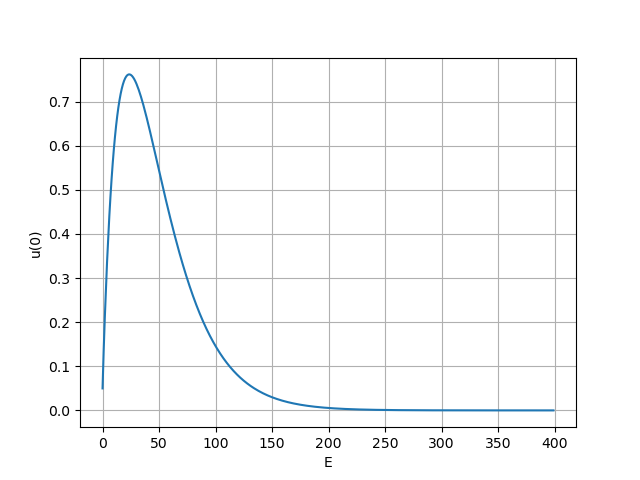
\includegraphics[width=.9\linewidth]{/home/chilkuri/Documents/codes/python/gscf/Fig-tmp.png}
\end{center}

\subsubsection{Plots}
\label{sec:org12bf04b}
\subsubsection{Main}
\label{sec:orgee794dc}
Make some figures.
\begin{center}
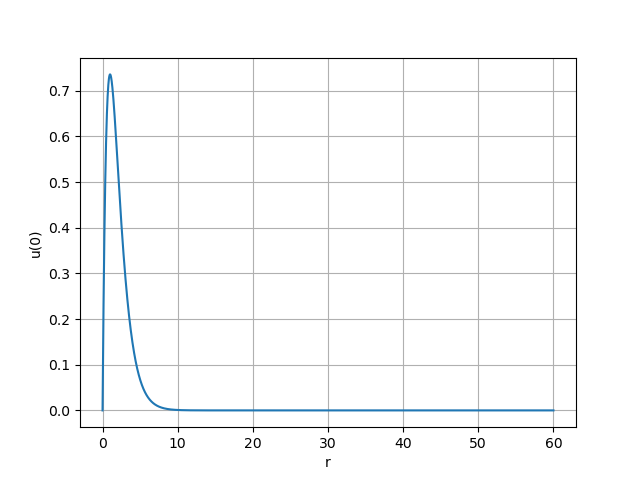
\includegraphics[width=.9\linewidth]{/home/chilkuri/Documents/codes/python/gscf/Fig-1.png}
\end{center}

\subsubsection{Solution of the SLP}
\label{sec:org8681974}

Here we have to search for the value of \(E\)
for which the BVP has the final conditions satisfied
i.e. \(u(r)=0\). This is done using the optimization
routine from \texttt{scipy}.

\subsubsection{Code}
\label{sec:org0e3ad7a}

The code is as follows

\begin{verbatim}
def get_energy_and_density(l,rr,z=1.,E=None, vectorfield=None, urf=None, tckur=None, fnx=None, tckfnx=None, fnc=None, tckfnc=None, xlim=0., ylim=-1.0E-6, isWF=True):
    dE = 0.51 # scan resolution to look for sign changes
    if E is None:
        E = -1.0 # starting energy

    if vectorfield is None:
        print("[get_energy_and_density] Error have to supply a vectorfield")
        return(0)

    if urf is None:
        def urf(x,tckur):
            return(0)

    def fn(e):
        u0s = shoot(e, rr, l=l, z=z, fn=urf, tckfn=tckur, fnx=fnx, tckfnx=tckfnx, fnc=fnc, tckfnc=tckfnc, vectorfield=vectorfield, xlim=xlim, ylim=ylim, isWF=isWF)[0]
        return(u0s)
    E_bound = root_scalar(fn, x0=E-dE, x1=E+dE).root
    _,u_bound,nrf,tck = shoot(E_bound, rr, l=l, z=z, fn=urf, fnx=fnx, tckfnx=tckfnx, fnc=fnc, tckfnc=tckfnc, tckfn=tckur, vectorfield=vectorfield, xlim=xlim, ylim=ylim, isWF=isWF)
    return(E_bound, u_bound, nrf, tck)
\end{verbatim}
\subsubsection{Testing}
\label{sec:org1b51349}
Test the functions.
\begin{verbatim}
numpoints=3200
stoptime=60.0
rr = np.array([stoptime * float(i+0.0001) / (numpoints - 1) for i in range(numpoints)])
E_bound,_,_,_ = get_energy_and_density(0,rr,vectorfield=vectorfield)
\end{verbatim}
\subsubsection{Main}
\label{sec:org66fab06}
Make figures.

\section{Helium atom}
\label{sec:org219ad1a}
Here we need to include the Hartree potential \(V_H\) which is the
repulsion between the two electrons

\[
V_H(\mathbf{r}) = \int dr'^3 n(\mathbf{r}')\frac{1}{\mathbf{r}-\mathbf{r}'}
\]

Where the \(n(\mathbf{r})\) is the density which is given as

\[
n(\mathbf{r}) = 2\sum_i^{N_{occ}} |\psi(\mathbf{r})|^2
\]

where we assume a closed shell spin singlet slater determinant.
In order to get the radial part of the density, we can use the
radial part of the wavefunction \(\psi(\mathbf{r})\) which is \(R(\mathbf{r})\).

\begin{align*}
n(r) &= 2\sum_i^{N_{occ}} |R(r)|^2 \\
n(r) &= 2\sum_i^{N_{occ}} \left |\frac{u(r)}{r}\right|^2 \\
\end{align*}


\subsection{Poisson equation}
\label{sec:org56b7f3a}

In order to calculate the Hartree potential Eq:\ref{Eq8}, we shall
transform it into an SLP which we can again solve using the
above methodology the solution of the Hydrogen atom.

\[
\nabla^2 V_H(\mathbf{r}) = -4 \pi n(\mathbf{r})
\]

This can again be transformed using the variable substitution
\(u(r)=rR(r)\) to a 1D equation.

\[
\frac{\partial^2 U(r)}{\partial r} = -4\pi r n(r)
\]

The fact that \(n(r)\) is simply \(R(r)^2\) by definition and the
fact that \(u(r)\) is normalized we can drop off \(4\pi\) to finally
obtain

\[
U''(r) = -\frac{u(r)^2}{r}
\]

This is the SLP that we need to solve to obtain the
hartree potential \(V_H(r)\).

\subsection{Solution}
\label{sec:org3f249d0}

The BVP Eq:\ref{Eq11} takes the following boundary conditions

\begin{align*}
U(0) &= 0\\
U(r_{max}) &= q_{max}
\end{align*}

where, \(q_{max}\) is the total charge. We shall use these conditions
in the shooting method to find the correct Hartree potential.

\[
q_{max} = \int_0^{max} \text{d}r\ u^2(r)
\]

\subsubsection{Vector Field}
\label{sec:orgdaf50c6}
\begin{verbatim}
def vectorfieldVH(w, t, p):
    """
    Defines the differential equations for the coupled spring-mass system.

    Arguments:
    w :  vector of the state variables:
              w = [x1,y1,x2,y2]
    t :  time
    p :  vector of the parameters:
              p = [m1,m2,k1,k2,L1,L2,b1,b2]
    """
    x1, y1 = w
    _, _, nrf, tck,_,_,_,_, z = p

    # Create f = (x1',y1'):
    f = [y1,
         -nrf(t,tck)*nrf(t,tck)/t
         ]
    return f
\end{verbatim}
\subsubsection{Testing}
\label{sec:orgd858ea1}
\begin{verbatim}
numpoints=400
stoptime=15.0
rr = np.array([stoptime * float(i+0.0001) / (numpoints - 1) for i in range(numpoints)])
qmax = 1.
xlim = qmax
ylim = 0
x1,urf,tckur = solve_SLP(fn=nrf, tckfn=tck, t=rr, xlim=xlim, ylim=ylim, vectorfield=vectorfieldVH)
\end{verbatim}
\subsubsection{Main}
\label{sec:org51caa7e}
\begin{center}
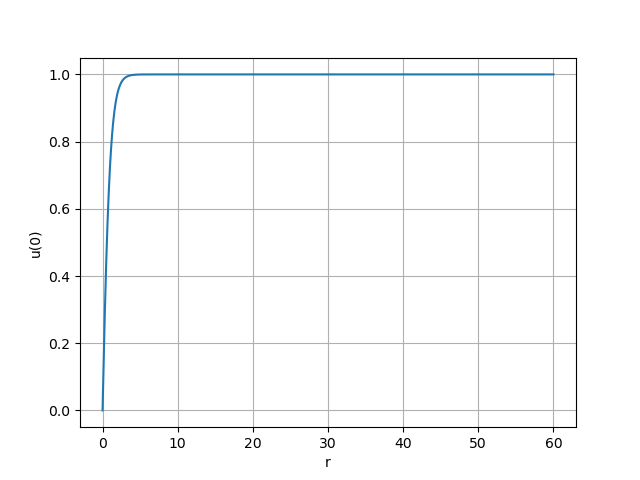
\includegraphics[width=.9\linewidth]{/home/chilkuri/Documents/codes/python/gscf/Figs/Fig-2.png}
\end{center}

\subsection{Self-consistent field cycle}
\label{sec:org07cac0b}

In order to find the solution, we need to perform a SCF loop
so that the energy stays constant.

In order to calculate the total energy, we now also need to
incorporate the Hartee potential

\[
E = 2 \epsilon - \int \text{d}r\ V_H(r) u^2(r)
\]


\subsubsection{Vector Field}
\label{sec:org607ff8f}
\begin{verbatim}
def vectorfieldHe(w, t, p):
    """
    Defines the differential equations for the coupled spring-mass system.

    Arguments:
    w :  vector of the state variables:
              w = [x1,y1,x2,y2]
    t :  time
    p :  vector of the parameters:
              p = [m1,m2,k1,k2,L1,L2,b1,b2]
    """
    x1, y1 = w
    e1, l1, urf, tckur, z = p

    # Create f = (x1',y1'):
    f = [y1,
         2*(l1*(l1+1)/(t)**2 - z/t - e1 + urf(t,tckur)/t)*x1
         ]

    return f
\end{verbatim}
\subsubsection{Calculate energy}
\label{sec:org5d50c29}
\begin{verbatim}
def calcEnergy(ei,urf,tckur,nrf,tck,t=None,stoptime=60.0,numpoints=3200):
    E = 2*ei
    if t is None:
        t = [stoptime * float(i+0.0001) / (numpoints - 1) for i in range(numpoints)]
    h = t[1]-t[0]
    VHl = np.array([urf(x,tckur)/x for x in t])
    Nr2 = np.array([(nrf(x,tck))**2 for x in t])
    eH = integrate.simps(VHl*Nr2, x=t)
    print(eH)
    E = E - eH
    return(E)
\end{verbatim}
\subsubsection{SCF cycle code}
\label{sec:org9f3270c}
\begin{verbatim}

stoptime=60.0
numpoints=3200
rr = np.array([stoptime * float(i+0.0001) / (numpoints - 1) for i in range(numpoints)])

# Get initial density
E_bound,_,nrf,tck = get_energy_and_density(0,rr,z=2.,E=-1.50,vectorfield=vectorfield)

# Get initial ur
qmax = 1.
xlim = qmax
ylim = 0.
x1,urf,tckur = solve_SLP(fn=nrf, tckfn=tck, t=rr, xlim=xlim, ylim=ylim, vectorfield=vectorfieldVH, isWF=False)
E0 = calcEnergy(E_bound, urf, tckur, nrf, tck)
print(E_bound, E0)

E_conv = []
dE_conv = []
E_conv.append(E0)
dE_conv.append(E0)
cnt = 0
Ediff = 10.
while cnt < 9 and abs(Ediff) > 1.E-4:

    # Get density
    E_bound,_,nrf,tck = get_energy_and_density(0,rr,z=2.,E=-1.50,vectorfield=vectorfield, urf=urf, tckur=tckur)
    # Get ur
    x1,urf,tckur = solve_SLP(fn=nrf, tckfn=tck, t=rr, xlim=xlim, ylim=ylim, vectorfield=vectorfieldVH, isWF=False)
    E1 = calcEnergy(E_bound, urf, tckur, nrf, tck,t=rr)
    #E1 = E_bound
    E_conv.append(E1)
    Ediff = abs(E0-E1)
    dE_conv.append(Ediff)
    print(f"Iter : {cnt} E = {E1} Diff = {Ediff} E_bound={E_bound}")
    E0 = E1

    cnt += 1
\end{verbatim}
\subsubsection{Main}
\label{sec:org05b6a3d}

\subsection{Figure}
\label{sec:org4aa9fe3}
\begin{center}
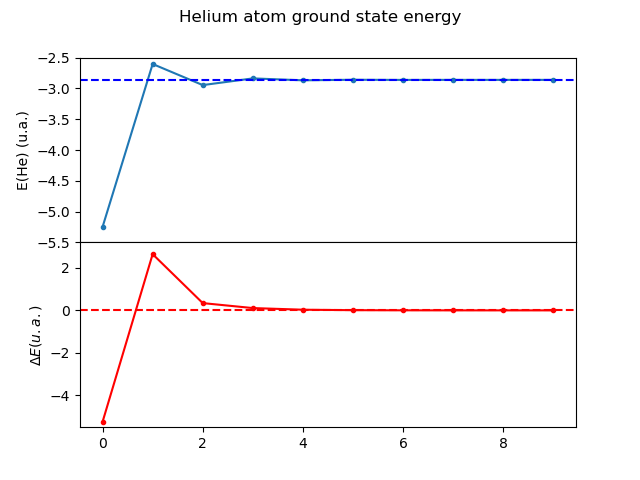
\includegraphics[width=.9\linewidth]{/home/chilkuri/Documents/codes/python/gscf/Figs/Fig-4.png}
\end{center}

\subsection{The local density Exchange potential}
\label{sec:org9d23a8d}

The Hartree potential used above is not the full potential since
we have substracted half of the electron density to take into
account the self-energy correction. However, if we take the
actual Hartree potential into account, the energy obtained is
very far from the exact energy.

In order to correct for this self interaction energy, we can use
the local density exchange potential (LDA). A simple functional
based on the electron gas is given as

\[
V_{\text{x}}(\mathbf{r}) = -\left( \frac{3}{\pi} \right )^{1/3} \times n^{1/3}(\mathbf{r})
\]


This potential is defined as the partial derivative of the exchange energy

\[
V_{\text{x}}[n](\mathbf{r}) = \frac{\partial}{\partial n (\mathbf{r})}E_{x}[n]
\]

And the exchange energy is given as

\[
E_{x}[n] = \int \text{d}^3 r \epsilon_{x}[n(\mathbf{r})]n(\mathbf{r})
\]

where the exchange energy density is given as

\[
\epsilon_{x}[n(\mathbf{r})] = -(3/4)(3/\pi)^{1/3} \times n^{1/3}(\mathbf{r})
\]

The local density exchange potential is derived from this local
energy density expression.

This local density based potential can correct for part of the self-energy error
in the Hartree potential. Note that here, and for the calculation for the
Hartree potential, the full density is to be taken. We can again
write this in terms of the radial function as

\[
V_{\text{x}}(\mathbf{r}) = -\left[ \frac{3u^2(r)}{2\pi^2r^2} \right ]^{1/3}
\]

and, using the above exchange energy, the total energy can then be
written as

\[
E = 2 \epsilon - \int \text{d}r\ V_H(r) u^2(r) + \frac{1}{2}\int \text{d}r\ V_{\text{x}}(r)u^2(r)
\]

The full equation the reads

\begin{align*}
\label{Eq16}
y &= \begin{pmatrix} u \\ u' \end{pmatrix}\\
y' &= \begin{pmatrix} u' \\ u'' \end{pmatrix} = \begin{pmatrix} u' \\ 2\left( \frac{l(l+1)}{r^2} -\frac{\mathcal{Z}}{r} + V_H + V_{\text{x}} - E \right) u \end{pmatrix}\\
\end{align*}

\subsubsection{Vector Field}
\label{sec:org8216bed}
\begin{verbatim}
def vectorfieldX(w, t, p):
    """
    Defines the differential equations for the coupled spring-mass system.

    Arguments:
    w :  vector of the state variables:
              w = [x1,y1,x2,y2]
    t :  time
    p :  vector of the parameters:
              p = [m1,m2,k1,k2,L1,L2,b1,b2]
    """
    x1, y1 = w
    e1, l1, urf, tckur, uxrf, tckurx, nrf, tck, z = p

    # Create f = (x1',y1'):
    f = [y1,
         2*(l1*(l1+1)/(t)**2 - z/(t) - e1 + 2*urf(t,tckur)/t + uxrf(t,nrf,tck) )*x1
         ]

    return f
\end{verbatim}
\subsubsection{Calculate energy}
\label{sec:orge0f3a58}
\begin{verbatim}
def calcEnergyVx(ei,urf,tckur,urxf,tckurx,nrf,tck,t=None,stoptime=60.0,numpoints=3200):
    E = 2*ei
    if t is None:
        t = [stoptime * float(i+0.0001) / (numpoints - 1) for i in range(numpoints)]
    VHl = np.array([urf(x,tckur)/x for x in t])
    Vxl = np.array([urxf(x,nrf,tck) for x in t])
    ur2 = np.array([(nrf(x,tck))**2 for x in t])
    eH = integrate.simps(VHl*ur2, x=t)
    ex = integrate.simps(Vxl*ur2, x=t)
    print((eH, (ex/2)))
    E = E - eH + (ex/2)
    return(E)
\end{verbatim}
\subsubsection{SCF cycle code}
\label{sec:org47ac654}
\begin{verbatim}

stoptime=60.0
numpoints=3200
rr = np.array([stoptime * float(i+0.0001) / (numpoints - 1) for i in range(numpoints)])

# Get initial density
E_bound,_,nrf,tck = get_energy_and_density(0,rr,z=2.,E=-2.50,vectorfield=vectorfield)

# Get initial ur
qmax = 1.
xlim = qmax
ylim = 0.
x1,urf,tckur = solve_SLP(fn=nrf, tckfn=tck, t=rr, xlim=xlim, ylim=ylim, vectorfield=vectorfieldVH, isWF=False)
E0 = calcEnergy(E_bound, urf, tckur, nrf, tck)
print(E_bound, E0)

def urxf(x,nrf,tck):
    numer = 3.*nrf(x,tck)*nrf(x,tck)
    denom = 2.*np.pi*np.pi*x*x
    return(-np.power(numer/denom,1/3))

E_conv = []
dE_conv = []
E_conv.append(E0)
dE_conv.append(E0)
cnt = 0
Ediff = 10.
while cnt < 30 and abs(Ediff) > 1.E-4:

    # Get density
    E_bound,_,nrf,tck = get_energy_and_density(0,rr,z=2.,E=-1.00,vectorfield=vectorfieldX, urf=urf, tckur=tckur, fnx=urxf, tckfnx=tckur, fnc=nrf, tckfnc=tck)
    # Get ur
    x1,urf,tckur = solve_SLP(fn=nrf, tckfn=tck, t=rr, xlim=xlim, ylim=ylim, vectorfield=vectorfieldVH, isWF=False)
    E1 = calcEnergyVx(E_bound, urf, tckur, urxf, tckur, nrf, tck, t=rr)
    #E1 = E_bound
    E_conv.append(E1)
    Ediff = abs(E0-E1)
    dE_conv.append(Ediff)
    print(f"Iter : {cnt} E = {E1} Diff = {Ediff} E_bound={E_bound}")
    E0 = E1

    cnt += 1
\end{verbatim}
\subsubsection{Main Shoot}
\label{sec:org601e5a0}
\begin{center}
\includegraphics[width=.9\linewidth]{/home/chilkuri/Documents/codes/python/gscf/Fig-tmp5.png}
\end{center}

\subsubsection{Main}
\label{sec:org461cfc3}

\subsection{Figure}
\label{sec:orge35b1a7}
\begin{center}
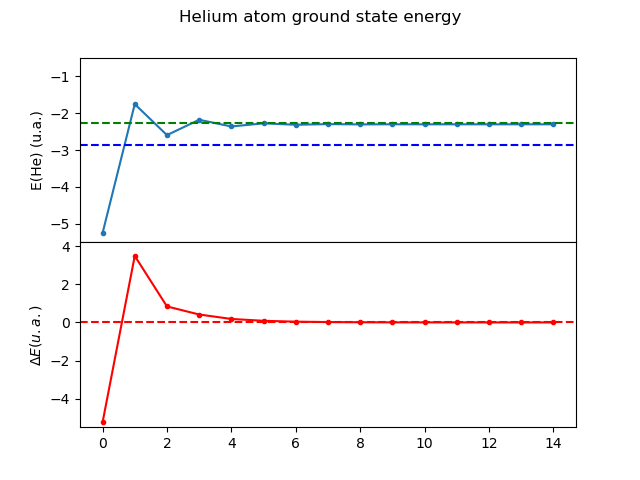
\includegraphics[width=.9\linewidth]{/home/chilkuri/Documents/codes/python/gscf/Figs/Fig-6.png}
\end{center}
\end{document}
